\section{Diseño del controlador}

\subsection{Control por realimentación de estados}

Gracias al observador de Luenberger desarrollado en la Sección~\ref{sec:obs}, se tiene acceso a estimaciones de rápida convergencia y bajo ruido de todas las variables de estado del sistema. Esto permite realizar un control por realimentación de estados, es decir, diseñar un controlador que cumpla con la siguiente relación de control
\begin{equation*}
    u_k = K \widehat{\mathbf{x}_k},
\end{equation*}
donde $K$ es una matriz de, en nuestro caso particular, $1\times4$. La misma se determina por \emph{pole placement}, utilizando un procedimiento similar al de los polos del observador.

\subsubsection{Diseño del controlador}

En un principio, el control se realizará con el único objetivo de estabilizar al sistema alrededor del punto de equilibrio. Es decir, no habrá una referencia.

Si se utilizaran los estados reales ($\mathbf{x}_k$) en lugar de los observados ($\widehat{\mathbf{x}_k}$), se tendrá
\begin{equation*}
    \mathbf{x}_{k+1} = (A_d + B_d K) \mathbf{x}_k,
\end{equation*}
por lo que ajustar $K$ permite colocar los polos del controlador en el lugar deseado, para conseguir una respuesta temporal acorde. Puede demostrarse que el reemplazo del vector $\mathbf{x}_k$ por su versión observada no mueve los polos del controlador, sino que agrega a la dinámica las singularidades pertenecientes al observador. Si se eligen éstas más rápidas, la respuesta del sistema a lazo cerrado estará aún dominada por los polos del controlador.

Para la elección de los polos del controlador, inicialmente se tomaron de forma tal que sean más lentos que los del observador, para que el control se base en estimaciones precisas de las variables de estado. En particular, se eligieron los polos continuos la mitad de lentos que los polos del observador. Dado que estos polos iniciales resultaron en un control vibrante, se decidió reducir por prueba y error los polos que involucran a las derivadas de las variables medidas, lo que se traduce en una menor dependencia de la acción de control a las variables ruidosas.

Los polos discretos del control por realimentación quedaron en
\begin{align*}
    p_1^{(C,d)} = 0.8040 + 0.1039j &&
    p_2^{(C,d)} = 0.9710 + 0.0470j \\
    p_3^{(C,d)} = 0.8040 - 0.1039j &&
    p_4^{(C,d)} = 0.9710 - 0.0470j.
\end{align*}
Los mismos equivalen a polos continuos en
\begin{align*}
    p_1^{(C,c)} = -10.4955 + 6.4285j &&
    p_2^{(C,c)} = -1.4117 + 2.4172j \\
    p_3^{(C,c)} = -10.4955 - 6.4285j &&
    p_4^{(C,c)} = -1.4117 - 2.4172j.
\end{align*}

La matriz de realimentación $K$ fue calculada por \emph{pole placement}. El resultado obtenido fue
\begin{align*}
    K = \begin{bmatrix}
        0.2533 && -0.0121 && -116.5175 && -30
    \end{bmatrix}.
\end{align*}

\subsubsection{Verificación}

Para la verificación del correcto funcionamiento del controlador, se simuló la respuesta a condiciones iniciales no nulas en la posición del carrito, midiendo todas las variables de estado del sistema. El resultado se comparó con la respuesta simulada, y se muestra en la Figura~\ref{fig:noff-vars}.

La Figura~\ref{fig:noff-theta} muestra el ángulo de la barra que se obtiene por simulación y que se estima utilizando el observador, para una condición inicial de posición de \qty{0.15}{\m} (y el resto de las variables inicialmente nulas). Vemos que el comportamiento simulado y observado son similares inicalmente, aunque hay un desfasaje de ángulo en estado estacionario que se debe al intento del controlador de reducir el error en estado estacionario.

La Figura~\ref{fig:noff-pos} muestra la posición del carrito simulada y observada. El comportamiento del sistema a lazo cerrado presenta un ligero sobrepico, más marcado en el caso de la posición real, y además tiene un error no nulo en estado estacionario en el caso real debido a la fricción.

Las velocidades angular y lineal se muestran en las Figuras~\ref{fig:noff-omega} y~\ref{fig:noff-vel}. Los comportamientos estimado y simulado son cualitativamente similares. Se nota que la velocidad del carrito estimada tiene un valor no nulo al inicio debido a que el observador espera una posición inicial nula e intenta corregir con la medición de la condición inicial.

\begin{figure}[!htbp]
    \centering
    \begin{subfigure}{0.49\linewidth}
        \centering
        \includegraphics[width=\linewidth]{noff-theta.eps}
        \caption{Ángulo de la barra.}
        \label{fig:noff-theta}
    \end{subfigure}
    \begin{subfigure}{0.49\linewidth}
        \centering
        \includegraphics[width=\linewidth]{noff-pos.eps}
        \caption{Posición del carrito.}
        \label{fig:noff-pos}
    \end{subfigure}

    \begin{subfigure}{0.49\linewidth}
        \centering
        \includegraphics[width=\linewidth]{noff-omega.eps}
        \caption{Velocidad angular de la barra.}
        \label{fig:noff-omega}
    \end{subfigure}
    \begin{subfigure}{0.49\linewidth}
        \centering
        \includegraphics[width=\linewidth]{noff-vel.eps}
        \caption{Velocidad del carrito.}
        \label{fig:noff-vel}
    \end{subfigure}
    \caption{Estados simulados y estimados por el observador.}
    \label{fig:noff-vars}
\end{figure}


\subsection{Actualización de observador}
Se optó por ralentizar los polos del observador luego de la primera implementación del control por realimentación de estados con control integral. La razón de esto fue que la acción de control era muy ruidosa y oscilante en esta instancia y al modificar los polos deseados de todas las formas posibles y no obtener respuesta positiva la única opción restante era que el observador se encontraba siguiendo a la planta demasiado rápido. Se comprobó esto al estudiar más en profundidad su comportamiento, observado previamente en la \autoref{fig:obs-vars}, que ya se preveía que observaba muy rápidamente.

Se requería que el observador siga de manera mucho más suave a las variables, por lo que se partió de la base de disminuir la magnitud de los polos continuos deseados. En principio se fijaron en un valor levemente mayor al polo más rápido de la planta: los cuatro polos deseados rondando los $\SI{-12}{\radian\per\second}$ cuando el polo máximo es $\SI{11.7303}{\radian\per\second}$. Luego se ajustaron finamente los valores hasta obtener señales suaves como las observadas en la \autoref{fig:obs-vars-new}. 

Los polos discretos utilizados finalmente son:

\begin{align*}  
	p_1^{(o,d)} = 0.7900 &&
	p_2^{(o,d)} = 0.7867 &&
	p_3^{(o,d)} = 0.7851 &&
	p_4^{(o,d)} = 0.7831.
\end{align*}

Y la matriz de realimentación $L$ resultó en:
\begin{align*}
	L = \begin{bmatrix}
		 0.0003 & 0.0002\\
		-0.4655 & -0.0020\\
		0.0001 & 0.3918\\
		-0.0019 & 1.5908
	\end{bmatrix}.
\end{align*}


\begin{figure}[!htbp]
	\centering
	\begin{subfigure}{0.49\linewidth}
		\centering
		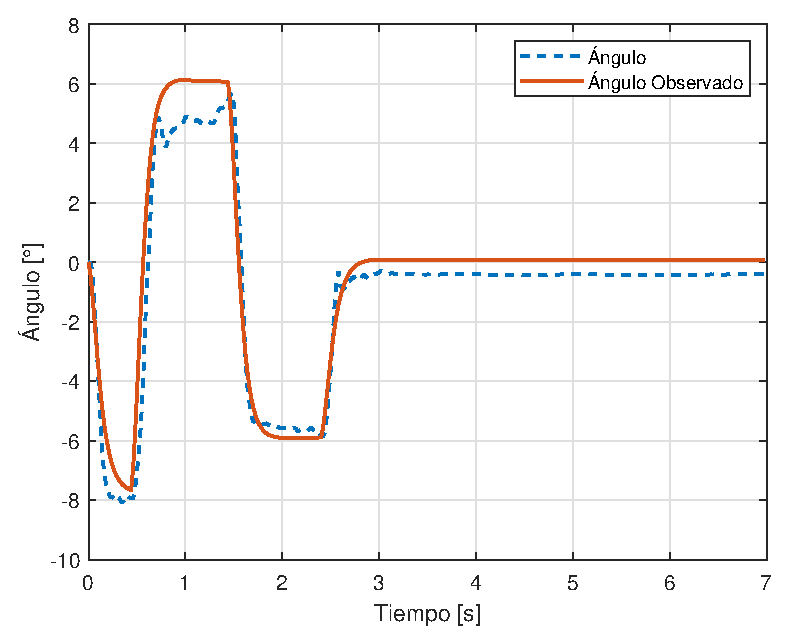
\includegraphics[width=\linewidth]{obs-theta-new.eps}
		\caption{Ángulo de la barra.}
		\label{fig:obs-theta-new}
	\end{subfigure}
	\begin{subfigure}{0.49\linewidth}
		\centering
		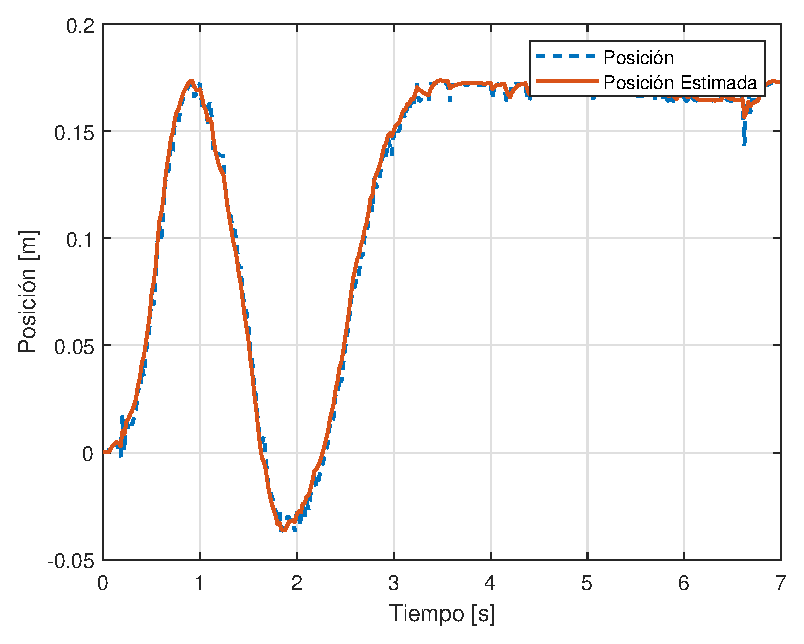
\includegraphics[width=\linewidth]{obs-pos-new.eps}
		\caption{Posición del carrito.}
		\label{fig:obs-pos-new}
	\end{subfigure}
	
	\begin{subfigure}{0.49\linewidth}
		\centering
		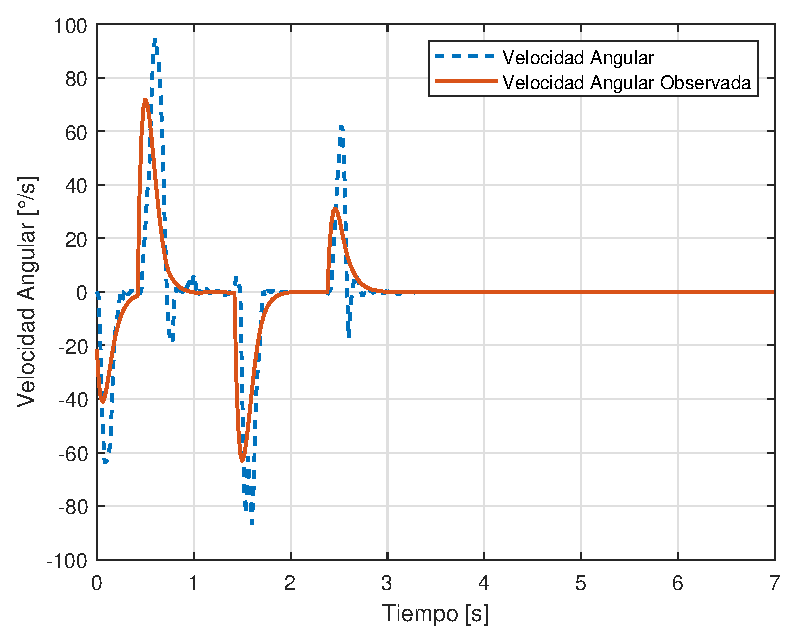
\includegraphics[width=\linewidth]{obs-omega-new.eps}
		\caption{Velocidad angular de la barra.}
		\label{fig:obs-omega-new}
	\end{subfigure}
	\begin{subfigure}{0.49\linewidth}
		\centering
		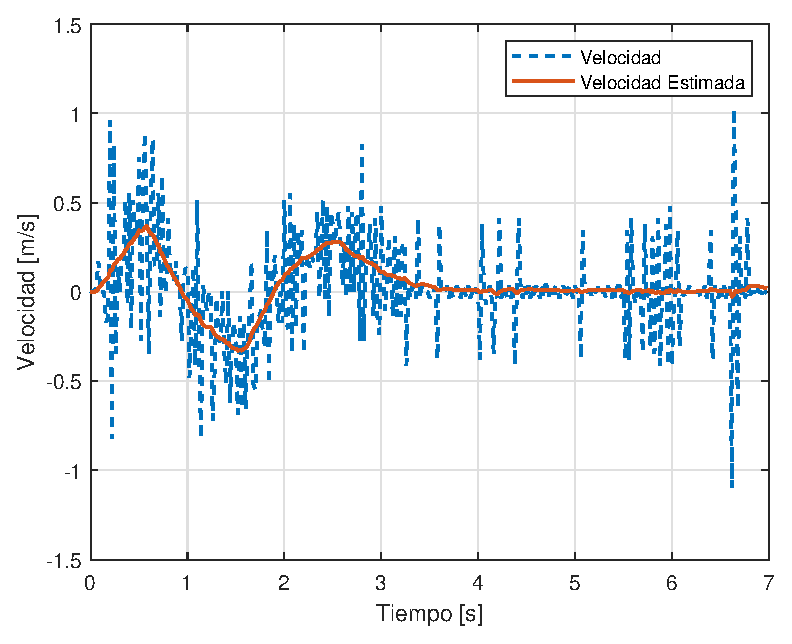
\includegraphics[width=\linewidth]{obs-vel-new.eps}
		\caption{Velocidad del carrito.}
		\label{fig:obs-vel-new}
	\end{subfigure}
	\caption{Estados medidos y estimados por el observador actualizado.}
	\label{fig:obs-vars-new}
\end{figure}

% vim: ts=4 sts=4 sw=4 et lbr
